\section{$V_4$ Symmetry}

Two commuting involutions act on the vertex set of $G_{60}$.
Together they generate a Klein four group

\[
V_4 = \mathbb{Z}_2 \times \mathbb{Z}_2 .
\]

The action partitions the vertices into $15$ orbits of size $4$.

\begin{figure}[h]
\centering
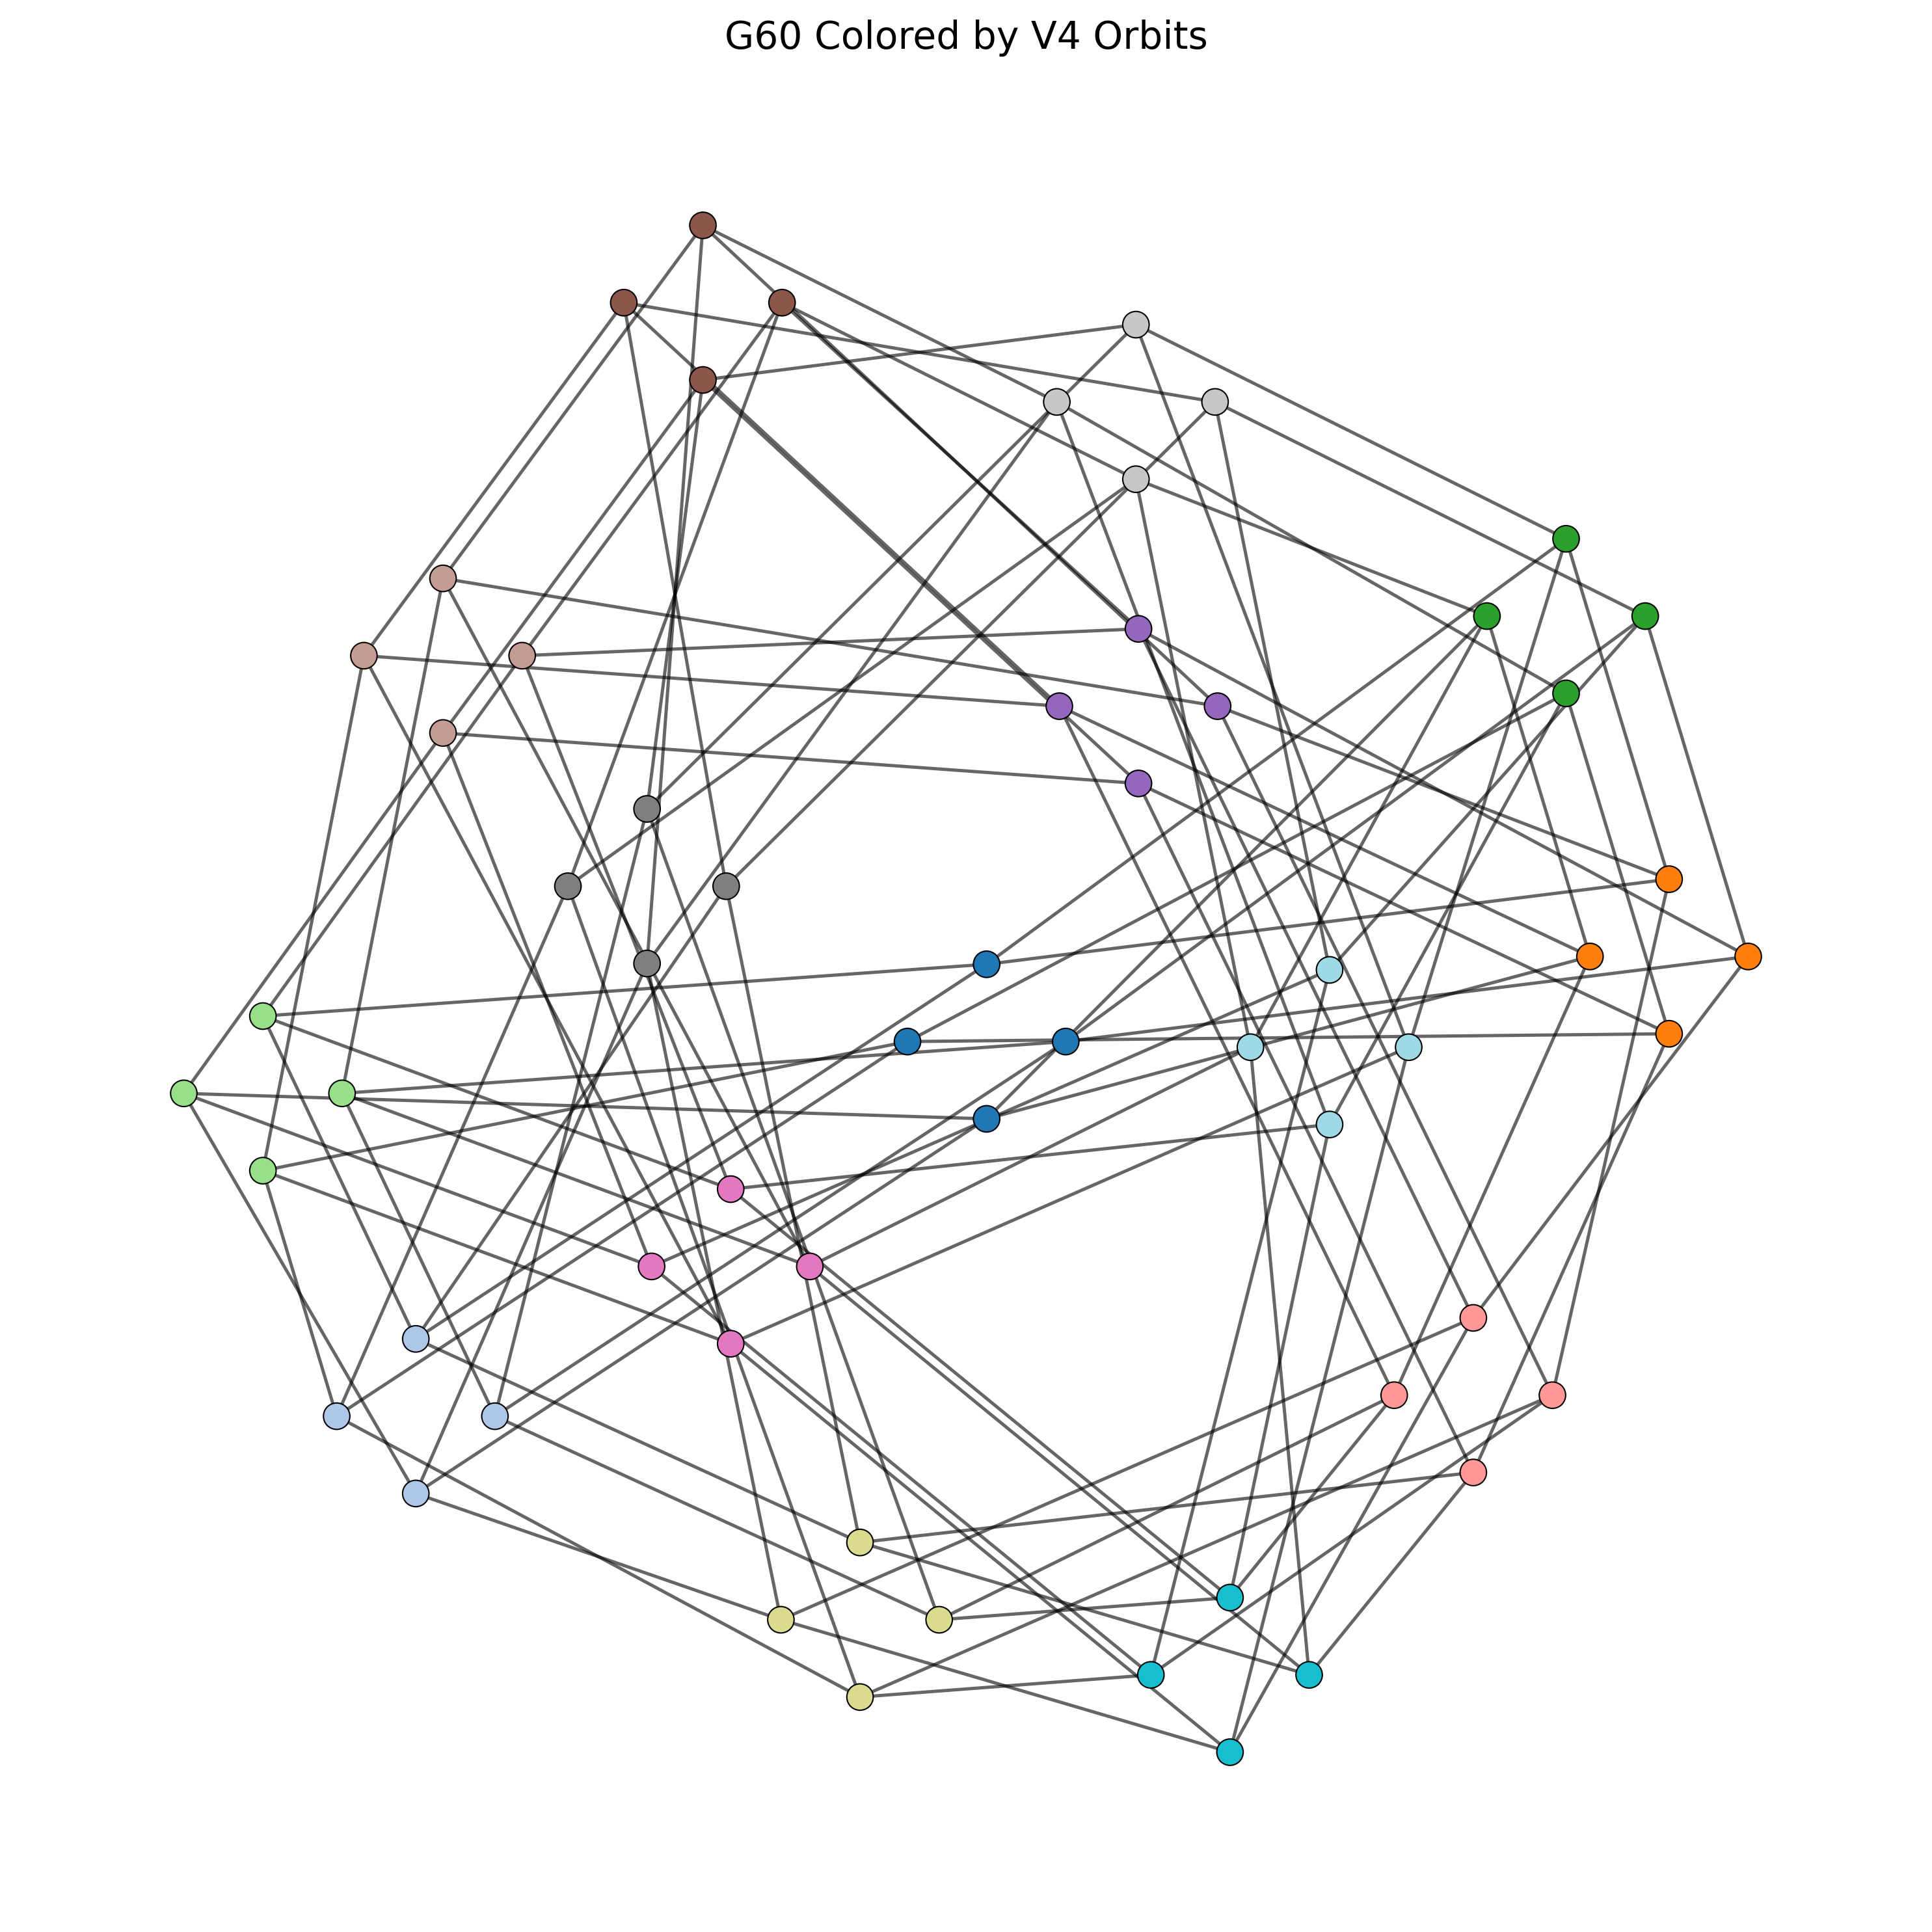
\includegraphics[width=0.75\linewidth]{figures/g60_v4_orbits.png}
\caption{$V_4$ orbit decomposition of the Thalean graph. Each color represents one orbit.}
\label{fig:v4_orbits}
\end{figure}

These orbits form the basis for the quotient construction described in the
next section.
